\section{General Statistics}
To get a broad overview of the dataset we decided to make some general numerical analysis of the dataset. In the part of the dataset, that we are analyzing there are \var{SizeDataset} playlists\footnote{Originally there are 1 million playlists. Due to limited processing power we had to reduce our analysis to a dataset of \var{SizeDataset} playlists.} with a total number of \var{unique_tracks} unique tracks by \var{artists_unique} artists in \var{albums_unique} albums. The total length of all playlist is \var{converted_total_duration} (hrs.:min.:sec.). The average number of tracks in one playlist is $\approx$ \var{approx_average_numtracks}\footnote{The exact number are \var{average_numtracks} tracks} tracks. The average duration of a playlist is \var{converted_average_duration}. This fits with the fact, that a track has an average duration of \var{converted_average_track_duration}.\footnote{Using the following calculation:\\$\text{average duration of track [ms]}\cdot\text{average number of tracks in a playlist}=\var{average_track_duration} \text{ ms}\cdot\var{average_numtracks}= \var{cal_average_playlist_duration} \text{ ms} = $ \var{converted_cal_average_playlist_duration}}

Knowing that the average number of tracks per playlist is \var{approx_average_numtracks}, we wanted to know how much these contribute to the total amount of unique tracks. For that we looked how the number of unique tracks changes when considering more playlists and plotted the results. To clearly show the relation, we changed the x-axis to a (square) root scale.


\definecolor{spotifygreen}{rgb}{0.12, 0.86, 0.384}
\begin{figure}[ht]
    \centering
    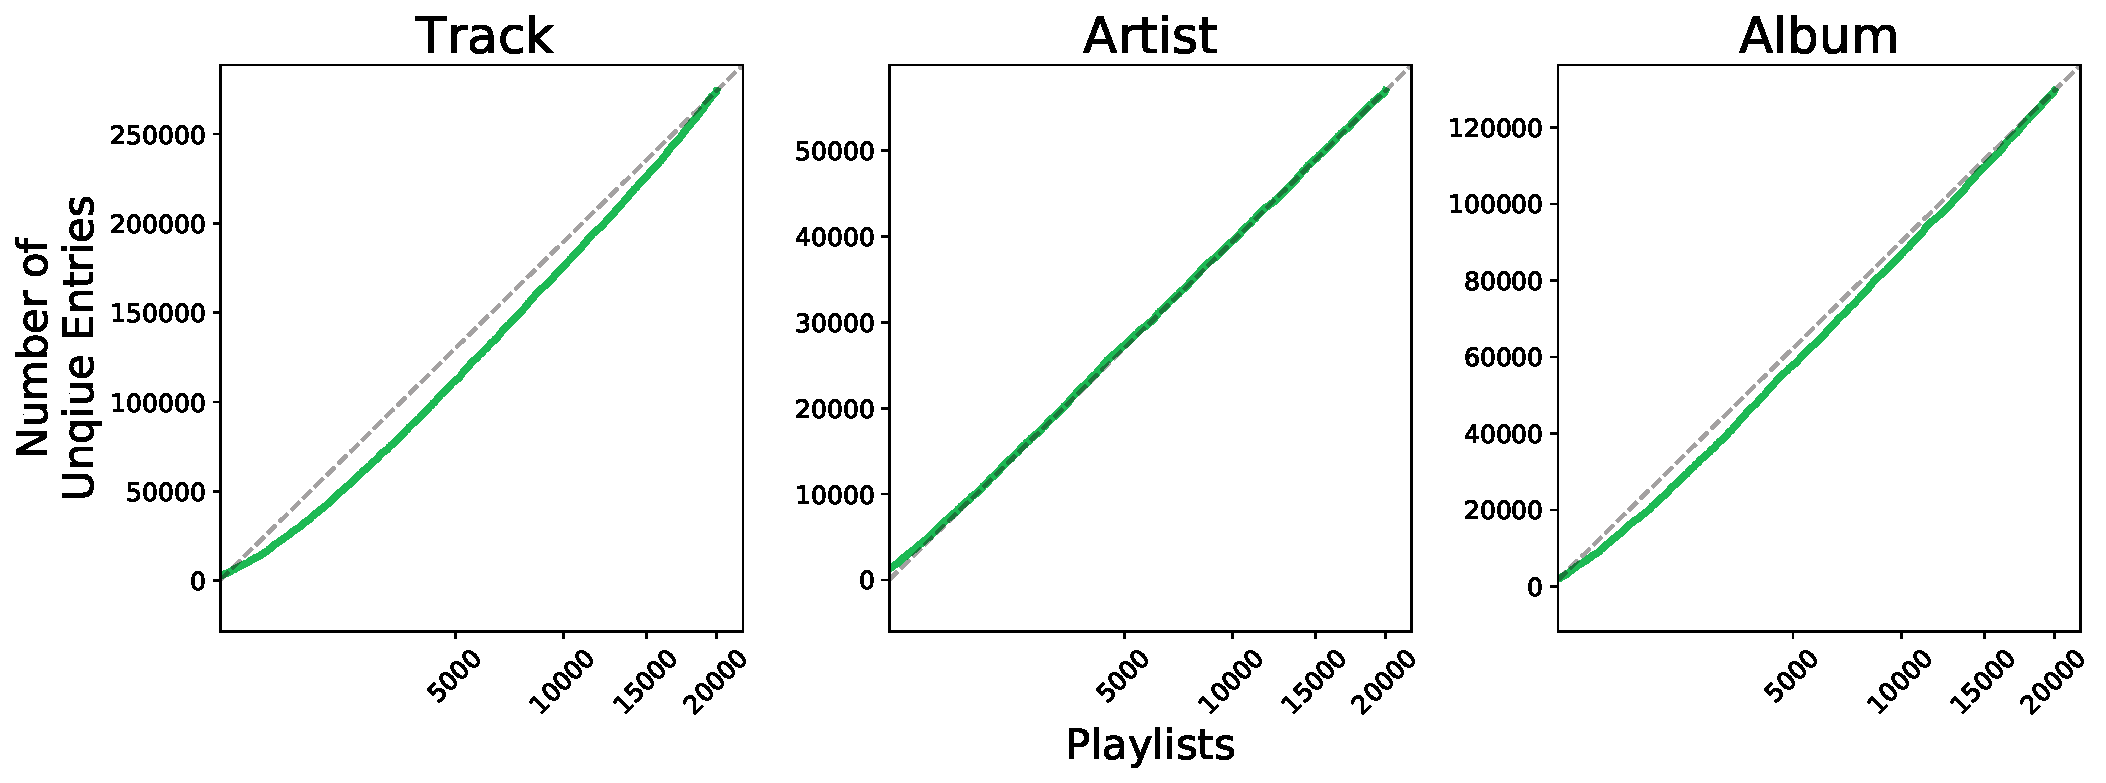
\includegraphics[width=\textwidth]{fig/unique_to_playlist.pdf}
    \caption{Line plot (\textcolor{spotifygreen}{---}) showing the relation between e.g. unique tracks and considered playlists, with a 45$^{\circ}$ line (\textcolor{gray}{- - -}) as baseline}
    \label{fig:unique_to_playlist}
\end{figure}

We now know that the number of unique tracks grows asymptotically to $\sqrt{x}*C$, where $C$ is the number of average added unique tracks and $x$ the number of playlists. This also holds for the number of artists and albums. 

To see what is mainstream, we got the most popular tracks, albums and artists and counted how often they were occurring in a playlist. The result is shown in tab. \ref{tab:popular}. When we compare this top 15 tracks with the top 15 of the "Year-end Charts Hot 100 Songs 2017" by billboard there is an overlap, of about $40 \%$.\footnote{The songs "Humble" by Kendrick Lamar, "Closer" by The Chainsmokers, "Bad and Boujee" by Migos, "Congratulations" by Post Malone, "XO TOUR Llif3" by Lil Uzi Vert and "Mask Off" by Future are in both top lists.}\citep{BillboardMedia} This is remarkable because the dataset is from January 2010 until November 2017 whereas the billboard top list is only resembling the year 2017.

\begin{table}[]
    \centering
    \caption{Top 15 Popular Tracks, Albums and Artists}
    \resizebox{\textwidth}{!}{%
    \begin{tabular}{clllllllll} \toprule
    Pos. & Occur. [$\%$]       & Track                 & Occur. [$\%$]       & Album                 & Occur. [$\%$]       & Artist                 \\
    \midrule
    1   & \var{top1track_occ}  & \var{top1track_name}  & \var{top1album_occ}  & \var{top1album_name}  & \var{top1artist_occ}  & \var{top1artist_name}  \\
    2   & \var{top2track_occ}  & \var{top2track_name}  & \var{top2album_occ}  & \var{top2album_name}  & \var{top2artist_occ}  & \var{top2artist_name}  \\
    3   & \var{top3track_occ}  & \var{top3track_name}  & \var{top3album_occ}  & \var{top3album_name}  & \var{top3artist_occ}  & \var{top3artist_name}  \\
    4   & \var{top4track_occ}  & \var{top4track_name}  & \var{top4album_occ}  & \var{top4album_name}  & \var{top4artist_occ}  & \var{top4artist_name}  \\
    5   & \var{top5track_occ}  & \var{top5track_name}  & \var{top5album_occ}  & \var{top5album_name}  & \var{top5artist_occ}  & \var{top5artist_name}  \\
    6   & \var{top6track_occ}  & \var{top6track_name}  & \var{top6album_occ}  & \var{top6album_name}  & \var{top6artist_occ}  & \var{top6artist_name}  \\
    7   & \var{top7track_occ}  & \var{top7track_name}  & \var{top7album_occ}  & \var{top7album_name}  & \var{top7artist_occ}  & \var{top7artist_name}  \\
    8   & \var{top8track_occ}  & \var{top8track_name}  & \var{top8album_occ}  & \var{top8album_name}  & \var{top8artist_occ}  & \var{top8artist_name}  \\
    9   & \var{top9track_occ}  & \var{top9track_name}  & \var{top9album_occ}  & \var{top9album_name}  & \var{top9artist_occ}  & \var{top9artist_name}  \\
    10  & \var{top10track_occ} & \var{top10track_name} & \var{top10album_occ} & \var{top10album_name} & \var{top10artist_occ} & \var{top10artist_name} \\
    11  & \var{top11track_occ} & \var{top11track_name} & \var{top11album_occ} & \var{top11album_name} & \var{top11artist_occ} & \var{top11artist_name} \\
    12  & \var{top12track_occ} & \var{top12track_name} & \var{top12album_occ} & \var{top12album_name} & \var{top12artist_occ} & \var{top12artist_name} \\
    13  & \var{top13track_occ} & \var{top13track_name} & \var{top13album_occ} & \var{top13album_name} & \var{top13artist_occ} & \var{top13artist_name} \\
    14  & \var{top14track_occ} & \var{top14track_name} & \var{top14album_occ} & \var{top14album_name} & \var{top14artist_occ} & \var{top14artist_name} \\
    15  & \var{top15track_occ} & \var{top15track_name} & \var{top15album_occ} & \var{top15album_name} & \var{top15artist_occ} & \var{top15artist_name} \\
    \bottomrule
    \end{tabular}}
    \label{tab:popular}
\end{table}